\chapter{Introduction}\label{chapter:intro}


\section{Cosmological preliminaries}
The currently accepted cosmological model describes space-time as a 4-dimensional Lorentzian manifold equipped with the Robertson-Walker metric \cite{carroll}
\begin{equation}\label{eq_ch1:RW_metric}
    \differential s^2=c^2\differential t^2-a(t)^2\left( \frac{\differential r^2}{1-kr^2}+r^2 \differential \Omega^2 \right),
\end{equation}
with $c$ the speed of light in vacuum, $a$ the scale factor, $k$ a curvature parameter and  $\differential \Omega$ the angular volume element in spherical coordinates. The scale factor is taken to be unity at present. At time $t$, a physical (proper) distance $l_\text{phy}$ is then related to a comoving distance $l_\text{com}$ by 
\begin{equation}\label{eq_ch1:phy_com_dis}
    l_\text{phy}=a(t)l_\text{cov}.
\end{equation}
The physical distance at time $t$ between an observer at $r=0$ and a point at $r$ is then
\begin{equation}\label{eq_ch1:def_com_len}
    l_\text{phy}=a(t)\int_0^r \frac{\differential r}{\sqrt{1-kr^2}}=a(t)\chi(r).
\end{equation}
The Robertson-Walker metric implies that for a radial luminous signal emitted at time $t_e$ and received at time $t_0$, we have
\begin{equation}
    \differential s^2=0 \implies \frac{\differential t_0}{a(t_0)}=\frac{\differential t_e}{a(t_e)}.
\end{equation}
As a consequence, the received frequency is redshifted according to
\begin{equation}
    1+z=\frac{\lambda_0}{\lambda_e}=\frac{\nu_e}{\nu_0}=\frac{a(t_0)}{a(t_e)},
\end{equation}
where $z$ is the redshift.

The time-dependence of physical distances in Equation \ref{eq_ch1:phy_com_dis} implies that an object whose comoving distance $\chi$ to an observer is constant recedes by following the Hubble flow according to
\begin{equation}\label{eq_ch1:hubble_law}
    v(t)=\dot{a}(t)\chi=\frac{\dot{a}}{a}a\chi=H(t)l_\text{phy},
\end{equation}
where $H(t)$ is known as the Hubble factor. Equation \ref{eq_ch1:hubble_law} is known as Hubble's law. At present time, $H(t_0)=H_0$ is referred to as Hubble's constant. For historical reasons, it is common to work with the reduced Hubble constant $h=H_0 [\text{km/s/Mpc}]/100$.
Note that, according to Equation \ref{eq_ch1:def_com_len}, and using the Robertson-Walker metric for a radial light signal, we obtain
\begin{equation}
    \differential \chi=\frac{c\differential t}{a}\implies \chi=\int_a^1\frac{\differential a}{a \dot{a}}=\int_0^z\frac{c \differential z}{H(z)}.
\end{equation}
As a consequence, the proper line element satisfies
\begin{equation}\label{eq_ch1:dl_over_dz}
    \differential \chi =\frac{c\differential z}{H(z)}=\frac{dl}{a(t)} \implies \frac{\differential l}{\differential z}=\frac{c}{(1+z)H(z)},
\end{equation}
which will be useful when integrating quantities along a line of sight. When working with such sightlines in spectroscopy, it is often advantageous to work with velocity units instead of redshifts (or proper distances). Differentiating Equation \ref{eq_ch1:hubble_law} and considering a slow varying Hubble factor around a mean redshift $\overline{z}$, we obtain the following useful expression:
\begin{equation}
    \differential v=H(\overline{z})\differential l=H(\overline{z})\frac{c\differential z}{(1+\overline{z})H(\overline{z})}=\frac{c\differential z}{1+\overline{z}}.
\end{equation}

The evolution of the scale factor (and hence of the redshift) with time is completely determined by the energy content of the universe through Einstein's field equation, which is known as Friedmann's equation in this context
\begin{equation}
    H^2=H_0^2\left( \Omega_\text{M} (1+z)^3+\Omega_\text{R} (1+z)^3 +\Omega_\Lambda + \Omega_K (1+z)^2 \right)=H_0^2E(z)^2,
\end{equation}
where the density parameters $\Omega$ are related to the physical densities of the components according to
\begin{equation}\label{eq_ch1:density_params}
    \begin{aligned}&\Omega_\text{M}&&=\quad\frac{8\pi G}{3H_0^2}\rho_{M0}\\&\Omega_\text{R}&&=\quad\frac{8\pi G}{3H_0^2}\rho_{R0}\\&\Omega_{\Lambda}&&=\quad\frac{8\pi G}{3H_0^2}\rho_{\Lambda}\\&\Omega_\text{K}&&=\quad-\frac k{H_0^2}\end{aligned}
\end{equation}
In Equation \ref{eq_ch1:density_params}, $\rho_\text{M}$ denotes the matter density of the universe, $\rho_\text{R}$ the radiation density, and $\rho_\Lambda$ the dark energy component. In the following, the values used for the cosmological parameters are $\Omega_m=0.308,\Omega_\Lambda=0.692,h=0.678,\Omega_b=0.0482,\sigma_8=0.829\mathrm{~and~}n=0.961, \Omega_\text{K}\approx 0$, as obtained from CMB measurements by the Planck Collaboration \cite{planck2014}. As we will discuss in Section \ref{sec:DM}, the current cosmological model $\Lambda$CDM include a cold dark matter component that dominates over baryonic matter. With the previous cosmological parameters, the matter and cosmological constant are equal when
\begin{equation}
    \Omega_\text{M}(1+z)^3=\Omega_\Lambda \implies z\approx 0.3.
\end{equation}
In consequence, at the redshift of interest for this work, $z\sim 4-5$, the universe is well-described as a matter-dominated universe.








\section{The intergalactic medium}\label{sec:IGM}
As the name suggests, the intergalactic medium (IGM) is the low-density part of the Universe content that permeates the space between halos and galaxies \cite{Mo2010}. The history of the IGM is closely related to the formation and evolution of galaxies, with multiple feedback mechanisms. For instance, IGM gas can aggregate and provide material to be captured by halos, while the radiation emitted by stars and quasars affects the state of the IGM. At sufficiently early times, all baryons were by definition part of the IGM, so the IGM represents the primordial material for galaxy formation. Since the IGM has very low densities, its properties are typically probed by the absorption of light coming from background sources, such as quasars. To give a rough overview of the properties of the IGM, its typical temperature is $\sim 10^4$ K, with peculiar velocities of $\sim 10-100$ km/s and neutral hydrogen column densities of $\sim 10^{12-17}$ cm$^{-2}$.

One of the most relevant processes in the IGM is ionisation. Consider the hydrogen recombination process:
$$p^+ + e^- \xleftrightarrow \ H +\gamma$$
The ionisation process has two main contributions: collisional ionisation and photo-ionisation.

Collisional ionisation tends to be non-dominant and is due to the collision of an energetic electron with a neutral hydrogen atom. Let $\Gamma_c$ be the collisional rate, so that the number of collisional ionisation per unit volume per unit time is $\Gamma_c n_{e^-}n_{HI}$. Photo-ionization is the dominant process and arises from an energetic photon colliding with a neutral hydrogen atom. Let $J$ be the flux of ionizing photons, then the number of photo-ionizations per volume per time is $\Gamma_i n_{HI}$ where 
\begin{equation}
    \Gamma_i=\int_{\nu_\mathrm{t}}^\infty\frac{4\pi J(\nu)}{ch_\mathrm{P}\nu}c\sigma(\nu)\operatorname{d}\nu
\end{equation}
and $\nu_t$ is the threshold frequency for ionizing photons (so, the Rydberg energy). If $\alpha$ is the recombination rate, the number of recombinations per time per volume is $\alpha n_{p^+}n_{e^-}$.
The equilibrium equation is the
\begin{equation}
    \alpha n_{p^+}n_{e^-}=\Gamma_i n_{HI}+\Gamma_cn_{e^-}n_{HI}  
\end{equation}
And so, the neutral hydrogen number density at equilibrium must be:
\begin{equation}
    n_{HI}=\frac{\alpha n_{p^+}n_{e^-}}{\Gamma_c n_{e^-}+\Gamma_i}
\end{equation}
Note that here $n_{p^+}$ is the density of free protons. If the gas is highly ionized we can take $n_{e^-}=n_{HI}+n_{p^+}\approx n_{p^+}$ and so, neglecting the collision part:
\begin{equation}
    n_{HI}=\frac{\alpha n_{p^+}^2}{\Gamma_i}
\end{equation}
In a dynamic universe, the equilibrium holds provided that the reaction rates are sufficiently large compared to the expansion time-scale $H^{-1}$. Since photo-ionization dominates, this can be expressed as 
\begin{equation}
    H^{-1}(z)<< \Gamma_i,
\end{equation}
where $\Gamma_i$ depends on the ionizing photon flux, and so depends on redshift.
















Considering that the IGM is made out of fully ionized hydrogen and helium, we have that:

\begin{equation}
    n_p=n_H+2n_{He} \hspace{2cm} n_n=2n_{He}
\end{equation}

The helium weight fraction is then defined as
\begin{eqnarray}
    Y=\frac{m_{He}}{m_{He}+m_H}\approx \frac{4n_{He}}{4n_{He}+n_H}=\frac{2n_n}{n_n+n_p}=\frac{2 n_n/n_p}{1+n_n/n_p}\approx 0.25 
\end{eqnarray}
The IGM also contains helium and a small fraction of metals, that contribute to its absorption properties.

We are generally interested in matter fluctuations of the IGM. Hence, we define the following quantity of interest, called the \emph{baryonic overdensity} field, as 
\begin{equation}
    \Delta =\frac{\rho}{\bar{\rho}}
\end{equation}
where $\rho(\bar{\rho})$ is the (mean) baryonic density. Let us recover the hydrogen density $n_H$ from the baryonic overdensity $\Delta$, the redshift $z$ and the density parameter $\Omega_b$.
First, suppose there is no overdensity so that $\Delta=1$ and the comoving density is homogeneous. Recall from the mean molecular weight section that
\begin{equation}
    \mu_H=\frac{1}{1-Y}=\frac{4}{3}=\frac{\rho_b}{m_pn_H}
\end{equation}
and that
\begin{equation}
    \rho_b=\frac{3H^2}{8\pi G}\Omega_b
\end{equation}
so that
\begin{equation}
    n_H=\frac{9H^2 \Omega_b}{32m_p\pi G} 
\end{equation}
Now, in a matter-dominated universe (for the redshifts we are interested in), the Friedmann equation states $H^2=H_0^2(1+z)^3$.
So, we obtain,
\begin{equation}
    n_H=\frac{9}{32m_p\pi G}H_0^2\Omega_b (1+z)^3
\end{equation}
and substituting values,
\begin{equation}
    n_H=1.7\cdot 10^{-7}(1+z)^3 cm^{-3}
\end{equation}
Now if, the hydrogen density is not homogeneous (that is, $\Delta \neq 1$), $n_H$ will be locally modulated by $\Delta$, so that
\begin{equation}\label{eq: delta and hydrogen density}
    n_H=1.7\cdot 10^{-7}(1+z)^3 \Delta \mathrm{cm}^{-3} .
\end{equation}
Since cosmological simulations typically produce as output the baryonic over density $\Delta$, we can use Equation \ref{eq: delta and hydrogen density} to recover the corresponding hydrogen density. The Lyman-$\alpha$ opacity can then be used to estimate the average neutral hydrogen fraction $x_\text{HI}$. The evolution of the observed Lyman-$\alpha$ optical depth indicates that the IGM is highly ionized at $z\lessapprox 5.5$, \cite{Becker_2001_GP_trough}, \cite{Ian_model_inde_reio}. The two main sources of UV ionising photons are believed to be young galaxies and quasars.




















Let us now describe how an intergalactic cloud (with no peculiar velocity) along the line of sight of a quasar affects its spectrum, allowing for a powerful probing mechanism of the IGM. Consider the situation illustrated in Figure \ref{fig_ch1:Lyman_alpha_diagram}, where a QSO at redshift $z_\text{QSO}$ emits photons, and consider the propagation of an emitted photon with rest-frame frequency $\nu_e$. Those photons are redshifted and are absorbed in $z_\alpha$ by a neutral hydrogen absorber with local number density $n(z_\alpha)$ producing an absorption feature in the flux at the rest-frame Lyman-$\alpha$ resonance $\lambda_\alpha \approx 1215$\r{A}. The unabsorbed photons are then redshifted and are detected by an observer at $z=0$ and a frequency $\nu_o$. The relationship between the frequencies mentioned above is then:
\begin{equation}
    \nu_o=\frac{\nu_e}{1+z_e}=\frac{\nu_\alpha}{1+z_\alpha} 
\end{equation}

\begin{figure}[t]
    \centering
    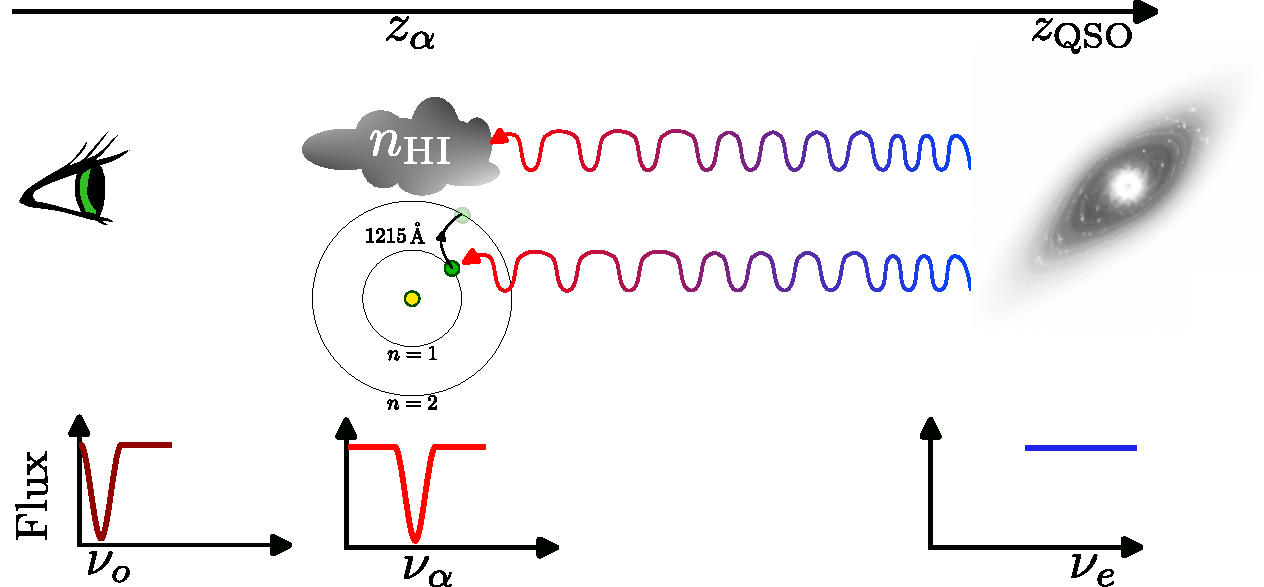
\includegraphics[width=1\linewidth]{img/lyman-alpha.pdf}
    \caption{Illustration of the Lyman-$\alpha$ absorption by neutral hydrogen at $z=z_\alpha$ in the line of sight of a QSO at $z=z_{\text{QSO}}$. In the observer's rest frame, the observed frequency is $\nu_o$. The associated frequency emitted by the QSO is $\nu_e$. }
    \label{fig_ch1:Lyman_alpha_diagram}
\end{figure}
We are interested in studying the effect of the Lyman-$\alpha$ absorbed at $z_\alpha$. The observed flux attenuation at the observed frequency $\nu_0$ is then expressed as $\exp(-\tau_\alpha)$, with $\tau_\alpha$ the Lyman-$\alpha$ opacity at the observed frequency, which depends on the observer's density and the Lyman-$\alpha$ cross-section $\sigma_\alpha(\nu)$. Observe now that since the Lyman-$\alpha$ cross-section is strongly peaked at the resonance $\nu_\alpha$, but can have a non-zero width, a nearby neutral hydrogen cloud might absorb photons at a redshift different to $z_\alpha$ that would have contributed to the observed flux at frequency $\nu_o$. With this consideration, we integrate over the line of sight to obtain the Lyman-$\alpha$ opacity at the observed frequency

\begin{equation}\label{eq_ch1:GP_integral}
    \tau_\alpha(\nu_o)=\int_o^{z_\text{QSO}} n_\text{HI}(z) \sigma_\alpha[\nu_o(1+z)] \differential z.
\end{equation}
If we now take $\sigma_\alpha(\nu)$ to be a Dirac delta centered at the resonance $\nu_\alpha$, and we integrate Equation \ref{eq_ch1:GP_integral} by using \ref{eq_ch1:dl_over_dz} we obtain

\begin{equation}\label{eq_ch1:GP_approx}
    \tau_\alpha(\nu_o)\approx \frac{cn_\text{HI}(z_\alpha)\sigma_\alpha}{H_0\Omega_\text{m}^{1/2} (1+z)^{1/3}},
\end{equation}
where now $\sigma_\alpha=4.5 \times 10^{-18}$cm$^2$ is to total Lyman-$\alpha$ cross-section.
Equation \ref{eq_ch1:GP_approx} is known as the Gunn-Peterson approximation for the Lyman-$\alpha$ opacity of the IGM \cite{GunnPeterson}. Equation \ref{eq_ch1:GP_approx} demonstrates that quasar spectra are a useful probe of the intergalactic neutral hydrogen density.





A more precise analysis of Equation \ref{eq_ch1:GP_integral} can be done if we do not approximate $\sigma_\alpha$ as a Dirac delta. Instead, we can include the two main broadening effects in the absorption cross-section: the natural broadening and the thermal broadening. The natural broadening is a result of quantum processes and generates a Lorentzian profile, while the thermal one is due to the microscopic Doppler effect of thermal motion and generates a Gaussian profile. The resulting combination of both the Lorentzian and Gaussian profiles is known as a Voigt profile. It is a non-analytical function with a Gaussian-like shape but heavier tails:
\begin{equation}\label{eq: Voigt}
    V(x,y)=\frac{Y}{\pi}\int_{-\infty}^{\infty}\frac{e^{-t^2}}{(x-t)^2+y^2} dt.
\end{equation}
The Lyman-$\alpha$ absorption cross-section described by the Voigt profile is then
\begin{equation}
    \sigma_\alpha(\nu)=\frac{cI_\alpha}{b\sqrt{\pi}} V\left(\frac{x(\nu-\nu_\alpha)}{b\nu_\alpha}, \alpha  \right),
\end{equation}
where $b=\frac{\sqrt{2k_BT}}{m_p}$ is the Doppler parameter at temperature $T$, $\nu_\alpha \approx 2.47\times 10^{15}$ Hz is the $Lyman-\alpha$ frequency, $I_\alpha \approx 4.45\times 10^{-18}$ cm$^{-2}$ is the total absorption cross-section \cite{Mo2010} and $\alpha$ is the recombination coefficient, which also depends on the temperature.
The Lyman-$\alpha$ cross-section is then peaked at the resonant frequency, and broadened by the temperature and the recombination rate. Now, consider a sightline of gas absorbing Lyman-$\alpha$ photons. Peculiar bulk velocities $v$ of the gas will add an additional Doppler effect in the cross-section as
\begin{equation}\label{eq:cross section}
    \sigma_\alpha(\nu)=\frac{cI_\alpha}{b\sqrt{\pi}} V\left(\frac{x(\nu-\nu_\alpha)}{b\nu_\alpha} +\frac{v}{b}, \alpha  \right).
\end{equation}
We can now integrate Equation \ref{eq:cross section} along the sightline to obtain the Lyman-$\alpha$ opacity $\tau$ as
\begin{equation}
    \tau = \int n(t)\sigma_\alpha(\nu_\alpha a(t_0)/a(t)) dt,
\end{equation}
where $n$ is the neutral hydrogen density and $t_0$ the emisison time.
Recalling that the comoving distance $x$ is related to redshift and time as 
\begin{equation}
    dx=\frac{c}{H(z)}dz=c(1+z)dt,
\end{equation}
we get that the Lyman-$\alpha$ optical depth $\tau$ can be obtained from the neutral hydrogen gas properties along the sightline as follows:
\begin{equation}\label{eq:lyman opacity}
    \begin{aligned}\tau(z_0)&=\frac{cI_\alpha}{\sqrt{\pi}}\int dx\frac{n_{\mathrm{H}}[x,z(x)]}{b[x,z(x)][1+z(x)]}\times V\left\{\frac{c[z(x)-z_0]}{b[x,z(x)](1+z_0)}+\frac{v[x,z(x)]}{b[x,z(x)]},\alpha\right\}\end{aligned}
\end{equation} 
where $n_\text{H}$ is the neutral hydrogen density, $b=\sqrt{\frac{2k_BT}{m_p}}$, $v$ is the peculiar velocity along the sightline, $m_p$ is the proton mass, $k_B$ is Boltzmann's constant, $\alpha$ is the recombination coefficient, $c$ is the speed of light, $I_\alpha$ is the total cross-section for Lyman-$\alpha$ absorption and $V$ is the Voigt function \cite{Choudhury_2001}. Since the Lyman-$\alpha$ flux $F=e^{-\tau}$ field depends on the properties of the absorbing gas, it contains information about the state of the IGM. The set of Lyman-$\alpha$ absorption features on the spectrum of a quasar is known as the Lyman-$\alpha$ forest. In Figure \ref{fig:forest} we show the spectrum of the quasar 1422+23, taken with the Keck HIRES instrument, and featuring a Lyman-$\alpha$ forest.

\begin{figure}[ht]
    \centering
    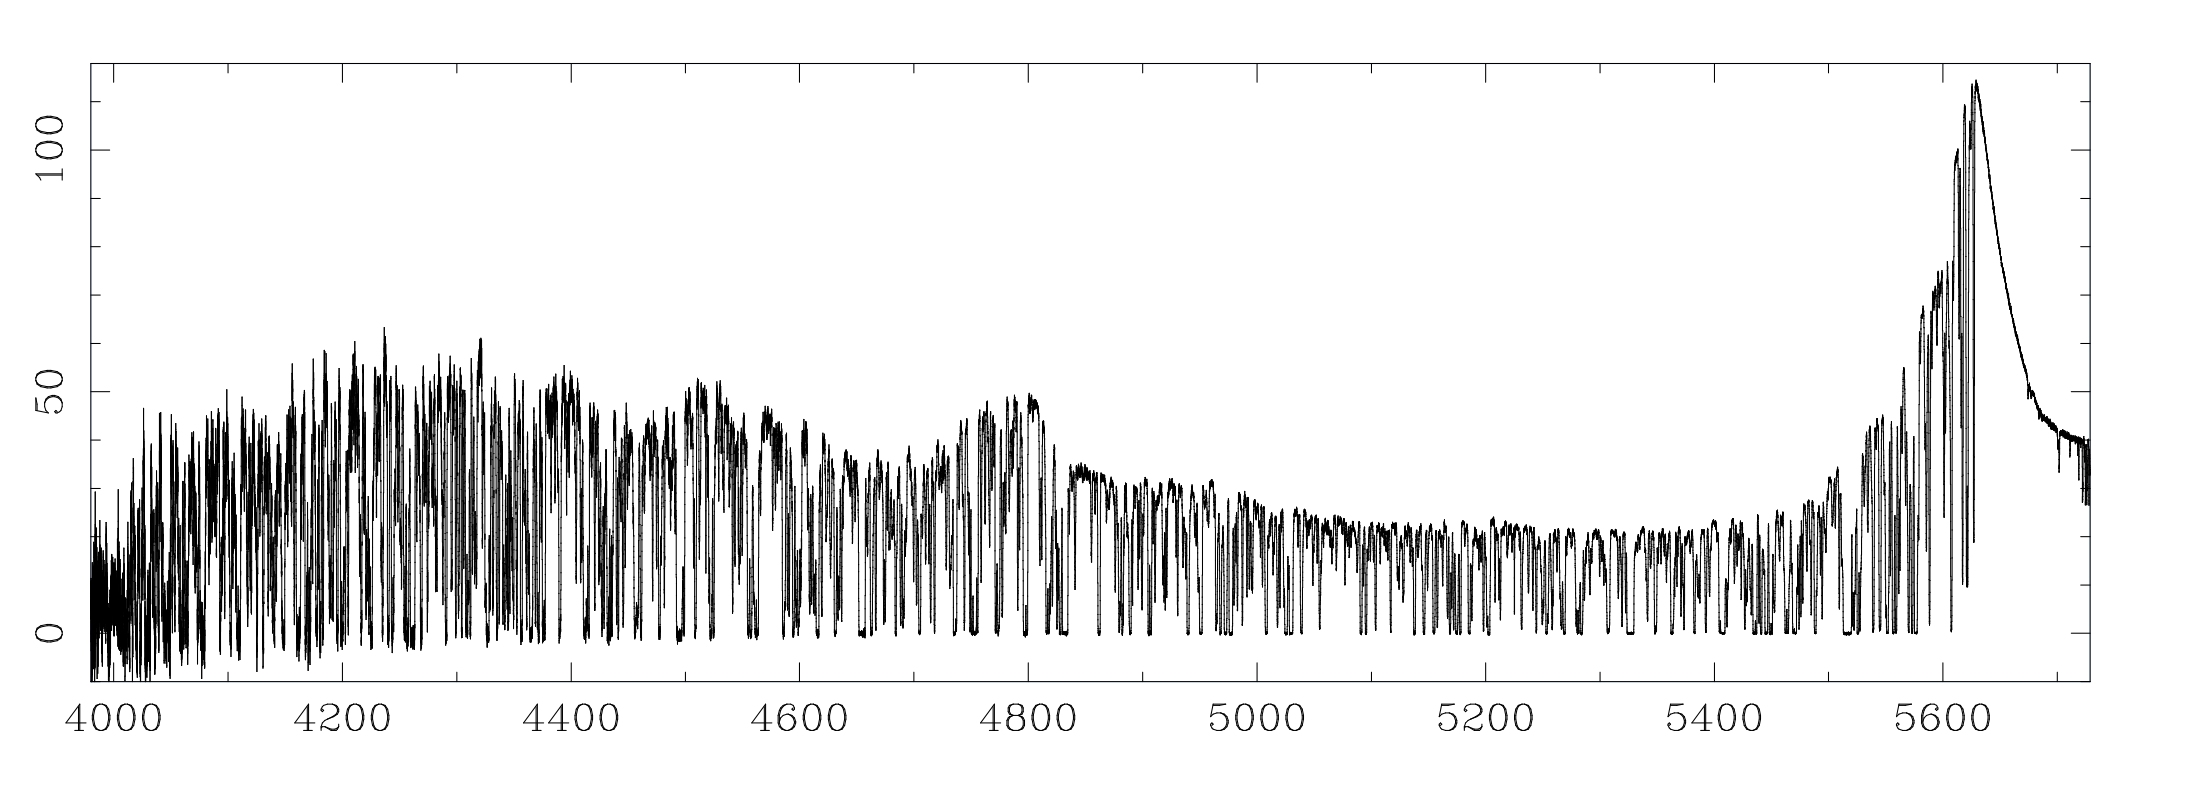
\includegraphics[width=1\linewidth]{img/ML/forest.png}
    \caption{High resolution (FWHM $\sim$ 6.6 km/s) spectrum of the $z = 3.62$ quasar 1422+23, taken with the Keck HIRES (signal-to-noise ratio $\sim$ 150 per resolution element, exposure time 25000 s). The horizontal axis is in units of observed wavelength in angstroms. Extracted from \cite{Rauch_1998}}
    \label{fig:forest}
\end{figure}

\section{Dark matter}\label{sec:DM}

Many aspects of the large-scale structure of the Universe can be understood by including a \emph{cold dark matter} (CDM) component that represents $\sim 26 \%$ of the critical density \cite{planck2014}. In the standard cosmological model, $\Lambda$CDM, dark matter is an important ingredient for structure formation in the Early Universe. However, its precise nature remains an outstanding problem both in cosmology and particle physics. With more exotic DM candidates, such as primordial black holes, heavily constrained, it is likely that DM consists of some undiscovered elementary particle(s) produced early in the history of the universe \cite{Villanueva_Domingo_2021}. There are multiple pieces of evidence supporting the CDM model, including the rotation curves of spiral galaxies and the kinematics of colliding clusters such as the Bullet cluster \cite{Navarro1996}, \cite{de_Blok_2008}.

According to the current paradigm \cite{Mo2010}, dark matter halos are the structures that host galaxies. They form through the gravitational collapse of non-linear perturbations in the primordial density field that serve as the first seeds for the formation of structures. Dark matter halos then grow by accreting material from their surrounding (such as the IGM). The properties of dark matter have then a direct influence on the properties of galaxies (formation, clustering, merging, etc.) and in the general distribution of matter in the Universe.

The evolution of the primordial fluctuations is not only determined by the gravitational clumping of matter but also by
the effect of random particle motions, which leads to a damping of the density peaks and perturbations. The scale at which this happens is set by the free-streaming length defined as the comoving distance travelled by a particle before a time $t$:
\begin{equation}
    \lambda_\mathrm{FS}=\int_0^t\frac{v(t')}{a(t')}dt'.
\end{equation}
$\Lambda$CDM models dark matter as pressureless and only interacting through gravity. Moreover, CDM decouples from the primordial plasma when it is already non-relativistic.
As a consequence, CDM has no significant amount of free-streaming, and (thermal)pressure does not hinder its clustering, which enables the formation of large hallos that can be as massive as $10^15$ M$_\odot$.

On large scales, the predictions of $\Lambda$CDM have been amply tested and are in good agreement with observations \cite{Dalal2002}, \cite{VanWaerbeke2004}, \cite{Eisenstein2005}. In contrast, on scales smaller than $\sim 10$ kpc, potential tensions between CDM predictions and observations might exist, including the ``core-cusp" problem related to the DM density profile in halos, or the ``too big to fail" problem linked to the number density of high-luminosity satellites in sub-halos \cite{Moore1994}, \cite{Boylan_Kolchin_2011}, \cite{Weinberg_2015}. Even if the inclusion of complex baryonic feedback processes can alleviate the aforementioned potential discrepancies, alternative models to CDM are worth exploring \cite{Vogelsberger2014}.  

As a consequence of these possible tensions, there have been a multitude of DM candidates to CDM. Such variations have included self-interactions \cite{Spergel2000} and fuzzy DM which leads to wave-like features in the density fields \cite{Hu2000}. Most alternative models retain the success of CDM on large scales while reproducing the desired features on smaller scales. Simulating how variations of CDM affect the evolution of structures in the Universe is highly non-trivial. Perhaps the simplest models that are viable to explore are warm(hot) dark matter WDM (HDM). Such candidates are usually classified according to their free-streaming scales. While for CDM particles $\Lambda_\mathrm{FS}$ is negligible at the scales of cosmological structure formation, for HDM models, such as light neutrinos, $\Lambda_\mathrm{FS}$ smooths out gravitational clustering even at galaxy cluster scales, leading to tight constraints on such models \cite{Hannestad_2004}. In between HDM and CDM, WDM offers an intermediate range of free-streaming scales that could potentially be compatible with the observed evolution of the Universe. In this work we focus on thermal relic WDM models, which include potential particles such as gravitinos or sterile neutrinos that were coupled to the original plasma in the Early Universe \cite{Viel_2005}. For such models, WDM is a particle of mass in the scale of the KeV. A WDM particle with a mass of $1$ KeV would have a free-streaming scale of $\Lambda_\mathrm{FS} \sim 0.3 Mpc$. In general, more massive particles are associated with smaller velocities and hence smaller $\Lambda_\mathrm{FS}$. The nature of WDM suppresses the total matter power spectrum on scales smaller than their free-streaming. That is, the less massive a WDM model is, the more the power spectrum is suppressed at small scales, and the more the density features of the density field are smoothed out.
To illustrate this process, consider Figure \ref{fig:villasenor_wdm}, which shows a simulated density field of the IGM as a function of redshift, and the WDM model mass. On the horizontal axis, the time evolution shows how gravity collapses dense regions into structures. On the vertical axis, the WDM free-streaming length suppresses small-scale clustering. 

\begin{figure}[ht]
    \centering
    \includegraphics[width=\textwidth]{img/ML/villa_wdm.png}
    \caption{Baryonic density plot of the IGM as a function of redshift, and the WDM model mass. On the horizontal axis, the time evolution shows how gravity collapses dense regions into structures. On the vertical axis, the WDM free-streaming length suppresses small-scale clustering. Extracted from \cite{Villasenor_2023}.}
    \label{fig:villasenor_wdm}
\end{figure}

Constraining WDM in the cosmological context involves understanding and determining which WDM model masses are compatible with the Universe we observe. Since the effect of WDM on structure formation is too complex, this process typically involves comparing simulations with observations: cosmological simulations are run for multiple WDM models, and the resulting properties are statistically compared to observations to rule out a certain range of masses. In Section \ref{chap:sherwood} we discuss how such simulations work and how WDM models are included in them.

Observations that have been used to constrain DM models include gravitational lensing \cite{Massey_2010} or the study of dwarf galaxies \cite{Calore_2018}. In this work, we focus on the Lyman-$\alpha$ forest that was introduced in Section \ref{sec:IGM}. As we have discussed, the properties of the Lyman-$\alpha$ forest depend on the properties of the IGM, and in particular on its matter distribution, which is directly linked with the WDM particle mass. Many efforts have been made to constrain WDM by comparing the Lyman-$\alpha$ forest generated by WDM models to the observed one in quasar spectra\cite{sherwood_wdm}, \cite{Villasenor_2023}, \cite{Viel_2005}.

\section{Structure of this work}
Building on previous efforts in the literature (most notably \cite{nasir2024deep}), in this work we explore the possibility of reconstructing the neutral hydrogen density field directly from the Lyman-$\alpha$ forest and whether such information can be used to constrain WDM. This reconstruction step involves careful analysis and represents a challenge at the frontier of the current efforts by the community. While the current state-of-the-art techniques extract information from the Lyman-$\alpha$ forest by using summary statistics, recovering the
non-observable physical fields of relevance would allow for the extraction of all the richness of information present in the forest. In particular, such techniques would allow for the mapping of the neutral hydrogen distribution in the Universe at the scales and redshifts where the forest is observable.

We begin in Section \ref{chap:sherwood} by exploring how WDM models affect the Lyman-$\alpha$ forest and the underlying neutral hydrogen field. For that purpose, we introduce a set of cosmological simulations that will be at the core of this work, the \texttt{SHERWOOD} simulation suite. We discuss the main aspects of such simulated data, including the cosmological code used in them. We conclude Section \ref{chap:sherwood} with a statistical analysis of the Lyman-$\alpha$ forest. Section \ref{chap: deep learning} is devoted to introducing the deep learning machinery used to reconstruct the neutral hydrogen density field from the Lyman-$\alpha$ forest flux. We begin by motivating the use of machine learning techniques and describing the basic concepts related and implementations related to such tools. Next, we discuss the motivation, architecture and implementation of the Bayesian neural network used in this regression task. We describe how we train the model using simulated data, evaluate its performance and robustness, and discuss some relevant questions about its internal dynamics. Armed with a machine learning pipeline that can reconstruct the neutral hydrogen density field from observed Lyman-$\alpha$ skewers, we are set to use this information in Section \ref{sec: inference pipeline} to constrain WDM. We discuss and implement a statistical pipeline to convert the recovered neutral hydrogen density field into WDM constraints. We extensively test this pipeline first on simulated data, from which we know the DM model used. Then, we turn our attention to real observational data and apply our technique to a set of quasar sightlines obtained from state-of-the-art spectrographs. We compare our results with the most up-to-date constraints in the literature, both in terms of tightness and efficiency in data usage.
